% Main document

\documentclass[english,12pt]{article}

% Für Deutsch
%\usepackage[utf8]{inputenc}
%\usepackage[ngerman]{babel}

% Packages
\usepackage{blindtext} % Lorem ipsum
\usepackage[a4paper,includeheadfoot,margin=2cm]{geometry} % Layout, showframe --> to see border
\usepackage{caption}
\usepackage[hidelinks]{hyperref} % links within the document and for clickable URLs
\usepackage{graphicx}
\usepackage[export]{adjustbox} % to beable to position images
\usepackage{amsmath} % equations
\usepackage{listings} % codeblocks
\usepackage{dirtytalk} % use quotations
\usepackage{titling} % So you can use theauthor
\usepackage[hybrid]{markdown} % Used to convert markdown
\usepackage{pdfpages} % Include pdf

\usepackage[backend=bibtex,style=ieee]{biblatex} % or verbose-trad2

\bibliography{source.bib} % add sources to source.bib file

% Image
\graphicspath{{img/}}
\usepackage{float} % Allows putting an [H] (place HERE & not where LaTeX wants to put)

% Header & Footer
\usepackage{fancyhdr}

\usepackage{siunitx} % Required for alignment
\sisetup{
	round-mode          = places, % Rounds numbers
	round-precision     = 2, % to 2 places
}
\usepackage{booktabs} % For prettier tables

% Document information
\title{ZHAWo - Platform Independent Timetable App}
\author{Bachmann Dominik, Visser Julian}

% Header & Footer
\pagestyle{fancy}
\fancyhf{}
\lhead{PA - HS 2018}
\chead{}
\rhead{ZHAWo}
\lfoot{}
\cfoot{\thepage}
\rfoot{}

\begin{document}

	\setlength{\parindent}{0in} % removes default indent of new paragraph

	% !TEX root = ba_doc.tex

%----------------------------------------------------------------------------------------
%	TITLE PAGE
%----------------------------------------------------------------------------------------
\begin{titlepage} % Suppresses displaying the page number on the title page and the subsequent page counts as page 1
	\newcommand{\HRule}{\rule{\linewidth}{0.5mm}} % Defines a new command for horizontal lines, change thickness here

	\center % Centre everything on the page

	%------------------------------------------------
	%	Headings
	%------------------------------------------------

	
\includegraphics[width=0.3\textwidth, left]{../../assets/zhawLogo.jpeg}\\[1cm]

	\textsc{\Large Projektarbeit IT}\\[0.5cm] % Major heading such as course name

	\textsc{\large HS 2018}\\[0.5cm] % Minor heading such as course title

	%------------------------------------------------
	%	Title
	%------------------------------------------------

	\HRule\\[0.5cm]

	%------------------------------------------------
	%	Logo
	%------------------------------------------------

	
\includegraphics[width=0.4\textwidth]{../../assets/zhawoLogo.png}\\[0.5cm]

	\textsc{\large \textbf{ZHAWo} \\[0.2cm]
									--- \\[0.3cm]}
	% Title of your document
\large{Platform Independent Timetable App}\\[0.5cm]


	\HRule\\[1cm]

	%------------------------------------------------
	%	Author(s)
	%------------------------------------------------

	\begin{minipage}{0.4\textwidth}
		\begin{flushleft}
			\large
			\textit{Authors}\\
			Bachmann Dominik \\
			Visser Julian % Your name
		\end{flushleft}
	\end{minipage}
	~
	\begin{minipage}{0.4\textwidth}
		\begin{flushright}
			\large
			\textit{Supervisor}\\
			Meier Andreas % Supervisor's name
		\end{flushright}
	\end{minipage}

	%----------------------------------------------------------------------------------------

	%------------------------------------------------
	%	Date
	%------------------------------------------------
	\vfill
	{\large\today} % Date, change the \today to a set date if you want to be precise

\end{titlepage}

	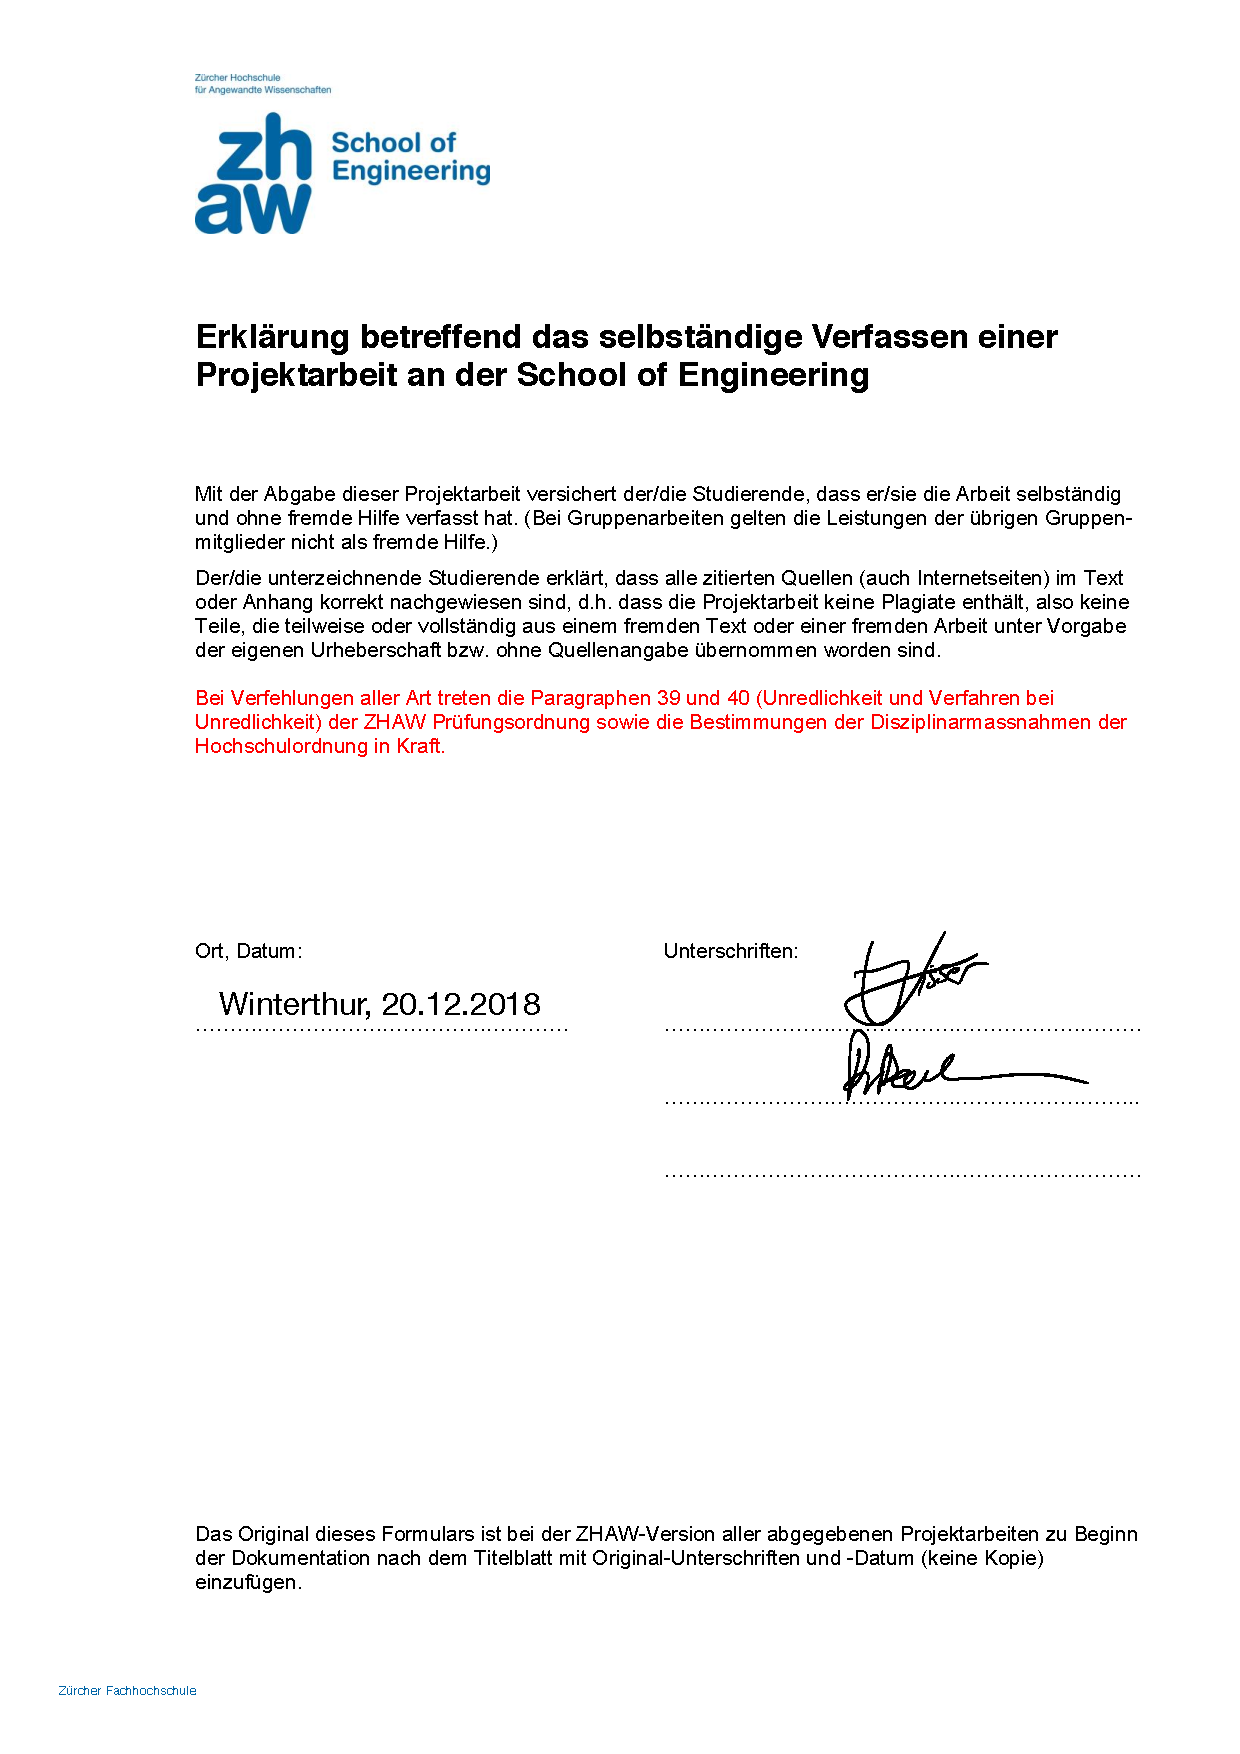
\includepdf{../../VorlagenZHAW/Erklaerung_PA.pdf}

	\pagenumbering{gobble}

	%Index
	\newpage
	\pagenumbering{roman}
	\tableofcontents
  \newpage
  \pagenumbering{arabic}

	% !TEX root = ba_doc.tex
\begin{abstract}
\begin{markdown}

\noindent With ZHAWo we want to provide students of the Zurich University of Applied Sciences (ZHAW) with a single application for their daily study tasks. Students need to be able to quickly look up their timetable, what lunch menus are available at their campus mensa and where a certain building or room can be found. While these functions are provided by the university's official app, we provide a consistent user experience among different platforms using Progressive Web App technologies. Additionally, with ZHAWo we provide students with an interface to search for free rooms. This function was previously provided by an app that is no longer available and was extensively used to find rooms for projects or study groups to work in environment less busy than the usually crowded official work spaces.

\noindent We also integrated news and events from the Verein Studierende ZHAW (vszhaw) into ZHAWo to provide students with easier access to information about events and services.

\noindent Using the JavaScript frameworks React for the frontend and Express for the backend in combination with Progressive Web App enables us to apply an agile development approach with fast prototyping of new features while still providing an application with the functionalities and feel that users expect from a native app. With this approach, we also avoid having to maintain multiple code bases for different platforms and mixing different technologies for frontend and backend. As a consequence, extending and improving the application's functionality can be done at a high velocity.

\end{markdown}
\end{abstract}

	\newpage

	% !TEX root = ba_doc.tex
\begin{markdown}
\section{Introduction} \label{introduction}

With ZHAWo \cite{OurHost}, our goal is to provide students with an improved application that allows them to access to their timetable and mensa menus in one single cross-platform application. Additionally, students can look for unoccupied rooms for both group projects and a quiet workspace. This functionality was - until about two years ago - provided by an Android application that was no longer maintained and eventually disappeared from the Google Play Store. While the official study rooms at, for example, the Technikum campus offer a space for both quiet work as well as group projects, in our experience as students it was very convenient to have a service to quickly look up free rooms without having to walk from room to room. Another feature ZHAWo provides is the integration of news \cite{VszhawNews} and events \cite{VszhawCalendar} of the vszhaw directly into the application. We aim to reduce the effort that is needed to stay up to date with the vszhaw and hope that both students and the vszhaw can profit from this.

Students of the Zurich University of Applied Sciences (ZHAW) have to visit multiple websites or use different applications on a daily basis in order to get information about their schedule, the offered menus in their campus mensa and events organized by the Verein Studierende ZHAW (vszhaw).

For their timetable, a student can either visit the official site \cite{Stundenplan} or use the official CampusInfo application for either Android \cite{AppAndroid} or iOS \cite{AppIOS}. The official site was designed for use on desktop browsers and is not optimised for responsiveness and display on phones. And while the official Android application is well maintained and offers a good user experience and a lot of additional features - such as direct access to public transport timetables and mensa menu plans - its iOS counterpart was seemingly lagging behind in development and at least at the start of this project did not offer the same user experience. The biggest issue with the iOS application was the lack of offline functionality. When a user's network cut out, even the timetable information that was previously loaded could no longer be accessed after navigating away. The iOS application has since received an update with a much improved design and offline functionality. This difference in quality and features is a common occurrence because the development of native applications requires two separate code bases for Android and iOS. 

When students want to check the mensa menus of their campus, they have the option of visiting the SV groups site \cite{SVSite} or to use the official Android or iOS application. These options suffered from the same issues as previously explained for the schedule and were also improved in a recent update.

The goal of this project was to build a production-ready application that can be distributed to and used by the students. The focus in this work is put on development of a PWA while evaluating advantages and disadvantages of using Progressive Web App technologies as well as user reception of our application.

By using Progressive Web Application (PWA) technologies \cite{PWA} in combination with JavaScript frameworks for both front- and backend, we achieve a consistent user experience on desktop, Android and iOS devices. We eliminated the issue of having to maintain separate code bases for different platforms while still being able to provide a native feel and functionality. PWA features such as offline caching of HTTP requests allow us to overcome previously mentioned issues with reliability on spotty networks. An additional advantage we gained by using PWA technologies and the same programming language across the full stack, was fast prototyping in an agile development process. Development of additional features and functionality can be achieved at a much faster rate with a single code base across all platforms.

\newpage

\end{markdown}

  \newpage

  % !TEX root = ba_doc.tex
\begin{markdown}
\section{Development} \label{development}

## Agile Approach

For the development of ZHAWo we used an iterative agile approach. The code base was managed on a single GitHub repository \cite{OurGithub} for both front- and backend. User stories were tracked using GitHub issues and the sprints were organised using GitHub project boards. We structured the development into sprints of 2 weeks. We regularly took feedback of other students and our own review of our practices and used technologies in our planning. The flexibility of using only JavaScript and PWA technologies enabled us to rapidly prototype new ideas without having to maintain two different code bases.
User stories were implemented and tested in feature branches and merged into the master branch as part of the sprint reviews. This practice ensured that we had stable iterations of the application to deploy for user feedback. A protocol of our sprint planning can be found on our GitHub wiki.

## Continuous Integration \& Deployment

For continuous integration we used Travis CI \cite{Travis} in combination with Codecov \cite{Codecov} to track test coverage. With good integration of both these tools into GitHub - for example reporting of build status and test coverage changes in GitHub comments on each pull request - we achieved good code and test quality across all feature implementations and sprints.
Each new iteration was deployed to a ZHAW server \cite{OurHost} and was directly pushed to our users on their next visit, without having to install an update through an app store as it would be the case with native applications.

## Primary Functions

To structure the development and implementation, we established four primary functions that our application should provide.

\begin{itemize}
  \item \textbf{Timetable}: A user can access their schedule and look up schedules of lecturers, classes, courses and rooms.
  \item \textbf{Menu plans}: A user can access menu plans of the different campus mensas across the ZHAW.
  \item \textbf{Room search}: A user can look for and find free rooms for a specific time-frame and location.
  \item \textbf{Student events}: A user can access vszhaw news and events to bring more attention to student parties and events.
\end{itemize}

\newpage

## Product Backlog

We divided each primary function into seperate smaller user stories to plan our sprints. Additionaly we have defined general user stories that are not directly related to any of the primary functions. All implemented user stories are listed in the following sections.

### General

\begin{itemize}
  \item \textbf{US01}: As a user I want to save my credentials/username
  \item \textbf{US02}: As a user I want the app to work even when I don't have network connection
  \item \textbf{US03}: As a user I want to switch between contexts (schedule, menus, room search, vszhaw)
\end{itemize}

### Timetable

\begin{itemize}
  \item \textbf{US10}: As a user I want to view my timetable/schedule for a day
  \item \textbf{US11}: As a user I want to view my timetable for a week
  \item \textbf{US12}: As a user I want to navigate to the current day
  \item \textbf{US13}: As a user I want to navigate between days when using the day view (timetable)
  \item \textbf{US14}: As a user I want to navigate between weeks (timetable)
  \item \textbf{US15}: As a user I want to navigate to a specific date in a month view (timetable)
  \item \textbf{US16}: As a user I want to view a specific room's timetable
  \item \textbf{US17}: As a user I want to view a specific class's timetable
  \item \textbf{US18}: As a user I want to view a specific course's timetable
  \item \textbf{US19}: As a user I want to view a specific person's timetable
  \item \textbf{US20}: As a user I want to have a detailed view of my events
\end{itemize}

\newpage

### Menu plans

\begin{itemize}
  \item \textbf{US50}: As a user I want to view the mensa menu for my campus for a day
  \item \textbf{US51}: As a user I want to view the mensa menu for my campus for a week
  \item \textbf{US52}: As a user I want to navigate to the mensa menu of the current day
  \item \textbf{US53}: As a user I want to navigate between days when using the mensa menu day view
  \item \textbf{US54}: As a user I want to navigate between weeks when using the mensa menu week view
  \item \textbf{US55}: As a user I want to navigate to a specific date in a month view (mensa menu)
  \item \textbf{US56}: As a user I want to see prices for all menus
  \item \textbf{US57}: As a user I want to navigate between menus of different days
  \item \textbf{US58}: As a user I want to view a specific mensa menu plan
\end{itemize}

### Room search

\begin{itemize}
  \item \textbf{US30}: As a user I want to find currently unoccupied rooms
  \item \textbf{US31}: As a user I want an overview of my campus with highlighted buildings where there are unoccupied rooms
  \item \textbf{US32}: As a user I want a floor plan of each floor per building with highlighted unoccupied rooms
  \item \textbf{US33}: As a user I want to navigate between buildings through the overview of my campus
  \item \textbf{US34}: As a user I want to navigate between floor plans of a building
  \item \textbf{US35}: As a user I want to see until when a room is unoccupied
  \item \textbf{US36}: As a user I want to filter my search to only show rooms that are unoccupied for at least x hours/minutes
\end{itemize}

### Student events

\begin{itemize}
  \item \textbf{US70}: As a user I want to view vszhaw blog posts/event announcements
  \item \textbf{US71}: As a user I want to see upcoming vszhaw events (f. ex. next party)
\end{itemize}

\end{markdown}

  \newpage

	% !TEX root = ba_doc.tex
\begin{markdown}
\section{Implementation} \label{implementation}

## Architecture

The architecture for ZHAWo consists of a frontend React \cite{React} web application and a backend server based on the Node.js \cite{Node} server framework Express \cite{Express}. The frontend communicates with the backend through a REST API. The backend server - apart from providing the REST API for the frontend - fetches timetable and menu data from the CampusInfo REST API provided by the ZHAW and fetches vszhaw news and calendar events through their RSS feed \cite{VszhawNews} and their calendar application \cite{VszhawCalendar}.

\bigskip
\bigskip

\begin{figure}[H]
  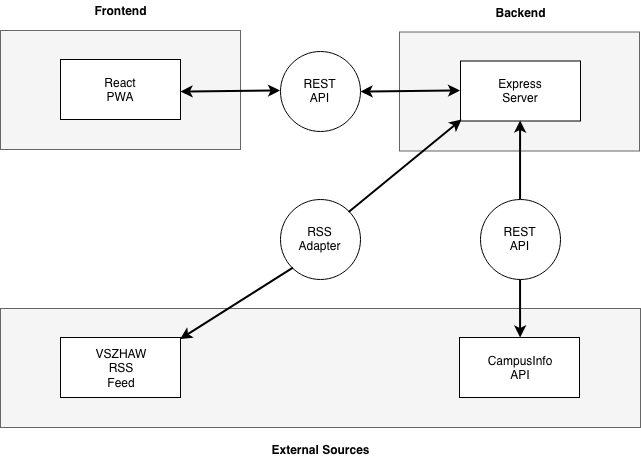
\includegraphics[width=14cm, center]{../../diagrams/applicationArchitecture.png}
  \captionsetup{width=13.5cm}
  \caption[Application Architecture Diagram]{\textbf{Application Architecture Diagram}: React frontend application communicating with backend Express server through a REST API. Express server fetches data from vszhaw RSS feed and calendar web application as well as the CampusInfo REST API for timetable and menu data.}
\end{figure}

\newpage

## Backend

The backend architecture consists of the following modules:

\begin{itemize}
  \item \textbf{Express server application}: Handles HTTP requests from frontend and redirection to persistance layer or third-party adapters.
  \item \textbf{Persistence layer}: Handles caching of more resource intensive requests such as room search. Implemented with basic file system using JSON file in the prototype. Can be extended by database if functionality requires.
  \item \textbf{REST API adapter}: Handles HTTP fetch requests to the CampusInfo API.
  \item \textbf{Vszhaw adapter}: Handles fetching of RSS feed and calendar events from vszhaw.
\end{itemize}

### Express Server Application

For the backend server application, we have chosen to use the framework Express \cite{Express} based on the Node.js \cite{Node} technology. The server is responsible to serve the frontend application and offers a REST API to get all the data the frontend needs. Most of the server logic handles redirecting user requests from the frontend to either persistence layer or the different API adapters and then serve the data. We have chosen to implement the backend with a JavaScript based framework so there is no technology difference between front- and backend. In the context of agile development in a small team, this allows for a fast implementation of features. A new feature often requires changes to both front- and backend, and by removing the need to switch context between different programming languages, we were able to maintain a good velocity throughout our sprints.

### Persistence Layer

In the scope of this project, there was no need to implement a full database for data persistence. The data for more resource intensive requests such as the search for free rooms is currently stored in JSON format directly in the servers file system. Less intensive requests such as timetables are delivered from CampusInfo in a format that only needs minimal modifications and are directly sent to the frontend without persistence.

However, should the need for a database later arise through new functionality, integration into the Express server application is already prepared.

### REST API Adapter

Most of the application data for ZHAWo is provided by the CampusInfo API. Since this is a third-party API provided by the ZHAW, we decided to implement an additional layer between our backend application core and the API. This insures that we are flexible to changes to CampusInfo.

### Vszhaw adapter

Similarly to the CampusInfo API adapter, the Vszhaw adapter provides an additional layer between our application and the RSS feed \cite{VszhawNews} of the vszhaw as well as the calendar web application \cite{VszhawCalendar}. This ensures that should the data received by this third-party feed and calendar application change, the changes needed to our application will be isolated to the adapter.

## Frontend

The frontend is made up of three main parts:

\begin{itemize}
  \item \textbf{React web application}: Handles presentation of data and user interaction.
  \item \textbf{REST API adapter}: Handles HTTP fetch requests to the backend.
  \item \textbf{Service worker}: Handles PWA functionality such as caching of data for offline use and installation to desktop or phone homescreen.
\end{itemize}

### React Web Application

For the presentation of the web application to the user, we used the React framework \cite{React}. React was originaly developed by Facebook and is one of the most popular UI libraries in web development. It is based on reusable components built with JSX, a syntax extension to JavaScript. We decided to use React because of its component based modularity, which works well with an agile development approach where multiple features need to be implemented simultaniously with little interference.

To handle the application data we chose to use the Flux design pattern \cite{Flux}. Using the Flux pattern ensures a unidirectional data flow from view components through actions into a single dispatcher into data stores, where the application data such as timetables and menu plans is handled. In Flux, the dispatcher is a singleton that directs the flow of data to ensure that updates do not cascade, which would lead to unpredictable behaviour. When a user interacts with a React view, the view sends an action through the dispatcher, which notifies the stores that hold the application’s data. When the stores change state, the view gets notified and changes accordingly \cite{Flux}.

### REST API Adapter

The data such as timetables, menu plans or lists of free rooms are provided by the backend REST API. To ensure modularity between front- and backend, we implemented an adapter module that handles all data requests to the backend. This practice allows easier adaptations to changes in API, as only the adapter would have to be changed, while the other parts such as the React application and service worker do not need to change.

The modularity this design choice provides - similarly to the modularity of React - goes well with the agile principle of fast prototyping of new ideas and features.

\bigskip

\begin{figure}[H]
  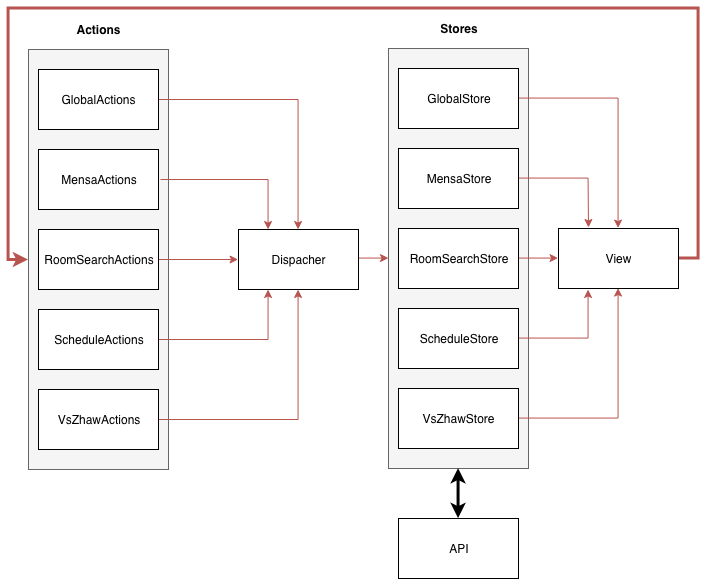
\includegraphics[width=14cm, center]{../../diagrams/flux.png}
  \captionsetup{width=13.5cm}
  \caption[Flux Pattern Diagram]{\textbf{Flux Pattern Diagram}: Unidirectional data flow from view components through actions }
\end{figure}

\bigskip

### Service Worker

The data for the frontend is provided by the backend REST API. All data received from HTTP fetch requests is cached using a service worker \cite{ServiceWorker}. By caching the application data, we ensure that the user can still access all the information that was already loaded once. It also improves the loading speed of ZHAWo, since resources that have been cached are first served from cache, before the data is requested by the backend. After the fetch request has completed the cache is updated. With regard to ,for example, a students schedule information, this practice makes a lot of sense since the actual data does not change often during the course of a semester.

In addition to offline caching, the service worker also allows users to install ZHAWo as a Progressive Web App (PWA) \cite{WhatIsPWA} to either their desktop or their phones homescreen.

These two features enables us to offer the experience of a native application while we avoid having to maintain separate code bases for each platform.

\end{markdown}



  \newpage

  % !TEX root = ba_doc.tex
\begin{markdown}

# Discussion

We were able to implement a prototype of ZHAWo as a Progressive Web App which covers all primary functions that were planned. Students can access their schedule, mensa plans and the news and event feed from vszhaw. Additionally, they can get a list of free rooms that can then be used as a distraction free work space. We were able to share the prototype with a small group of students and user feedback for our application was positive.

Using a full JavaScript technology stack for front- and backend and Progressive Web Apps has proven to work well with an agile development approach. While developing native applications, having to maintain different code bases can be awkward in combination with agile principles. The strength of the agile development approach that we have chosen is that we can prototype new features rapidly and can receive user feedback from both Android and iOS users immediately. In addition to that, not having to stay up to date with best practices, libraries and frameworks for different languages such as Java/Kotlin and Swift/Objective C for Android and iOS development respectively allowed us to implement new features at a faster pace.

While there are obvious advantages to building ZHAWo as a cross platform PWA, we have also identified some weaknesses. Installing an application not through the App Store or the Google Play Store is unexpected for most users. There are also some inconsistencies in support offered by different platforms. We attribute most of our issues to PWA technologies being relatively new and expect both support and users familiarity with the concept of PWAs to increase in the near future.

In a second part of this project, we aim to improve the user experience further and extend ZHAWo with more features.

\end{markdown}

  \newpage

	%\markdownInput{example.md}

	\section{Appendix}

	\listoffigures
  % \listoftables

	%\renewcommand\refname{Literaturverzeichnis} % rename --- für Deutsch
	\printbibliography % Uses source.bib to make ref table

\end{document}
